\chapter{Results}
\label{results}
While the problem istance is too big to find an optimal solution, the models have been given ample time to compute feasible qualitative routes. Unexpectedly, the subtour elimination model is less efficient than the polinomial model, even in smaller instances. Even more unexpectedly, the polinomial formulation seems to be more efficient than the custom Column Generational approach, finding better solutions in orders of magnitude less time.

We have run the two models on two datasets each: one for the forecasted data and the other for the real data.
The polynomial approaches have been time-limited by the memory of the calculator as they seem to consume far more than what the running computer had to offer, thus their time will be lower than those for column generation.
The results are displayed in Figure~\ref{fig:res-colgen-avg}, Figure~\ref{fig:res-colgen-real}, Figure~\ref{fig:res-poly-avg} and Figure~\ref{fig:res-poly-real}.


As can be observed, the polynomial model consistently yields superior results in significantly less time compared to our Branch and Price method. This observation is a testament to the impressive work done by the Gurobi team in developing Mixed Integer Programming (MIP) solving solutions that can efficiently handle even the most straightforward problem formulations.

It is worth noting, however, that we may have achieved even better results had we implemented more efficient subproblem formulations. With the benefit of hindsight, we recognize that given the number of clients required, a metaheuristic solution might have been a more appropriate approach. Nonetheless, the results obtained through our selected approach provide valuable insights into the problem and pave the way for further optimization efforts in the future.


\begin{figure}[tb]
    \centering
    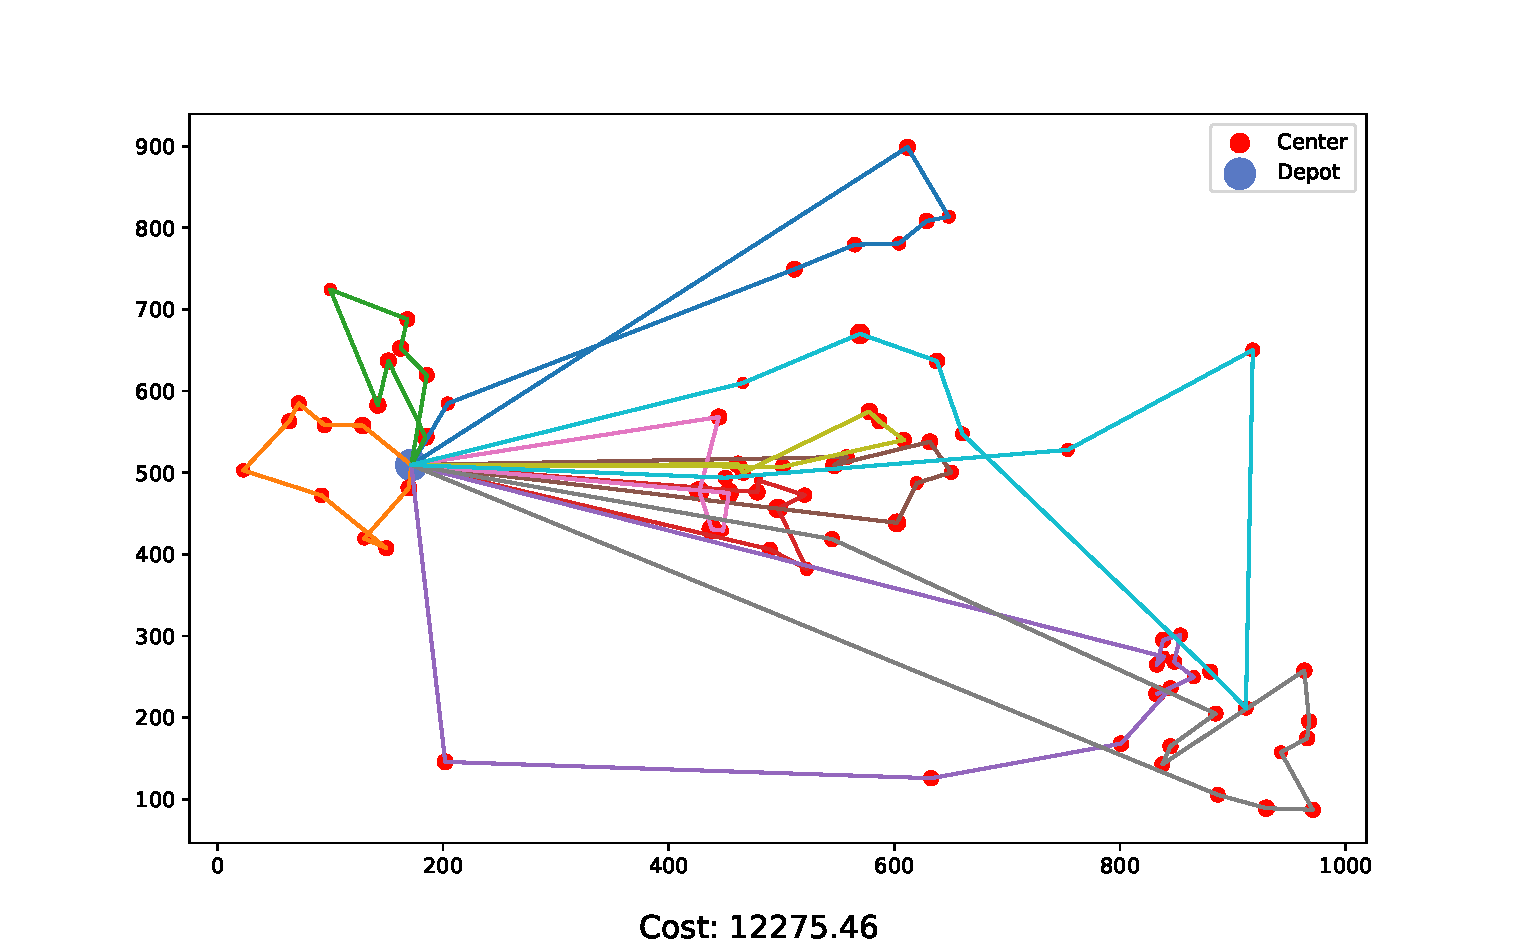
\includegraphics[width=1\columnwidth]{figures/results_colgen_avg.pdf}
    \caption{method: column generation, data: average, runtime: 11h}
  \label{fig:res-colgen-avg}
\end{figure}

\begin{figure}[tb]
    \centering
    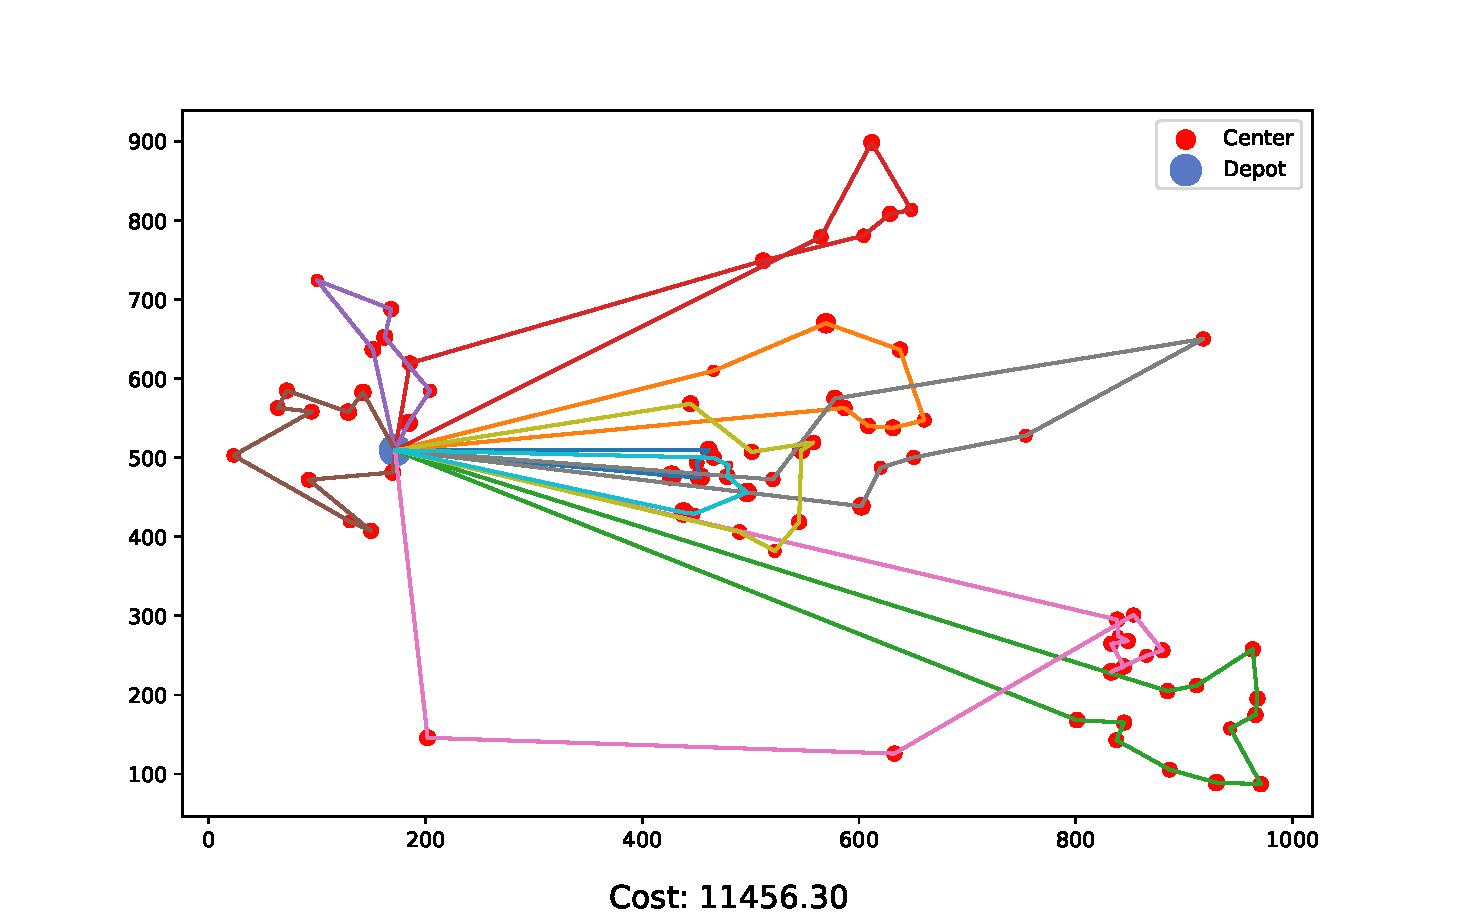
\includegraphics[width=1\columnwidth]{figures/results_colgen_real.pdf}
    \caption{method: column generation, data: real, runtime: 22h}
  \label{fig:res-colgen-real}
\end{figure}

\begin{figure}[tb]
    \centering
    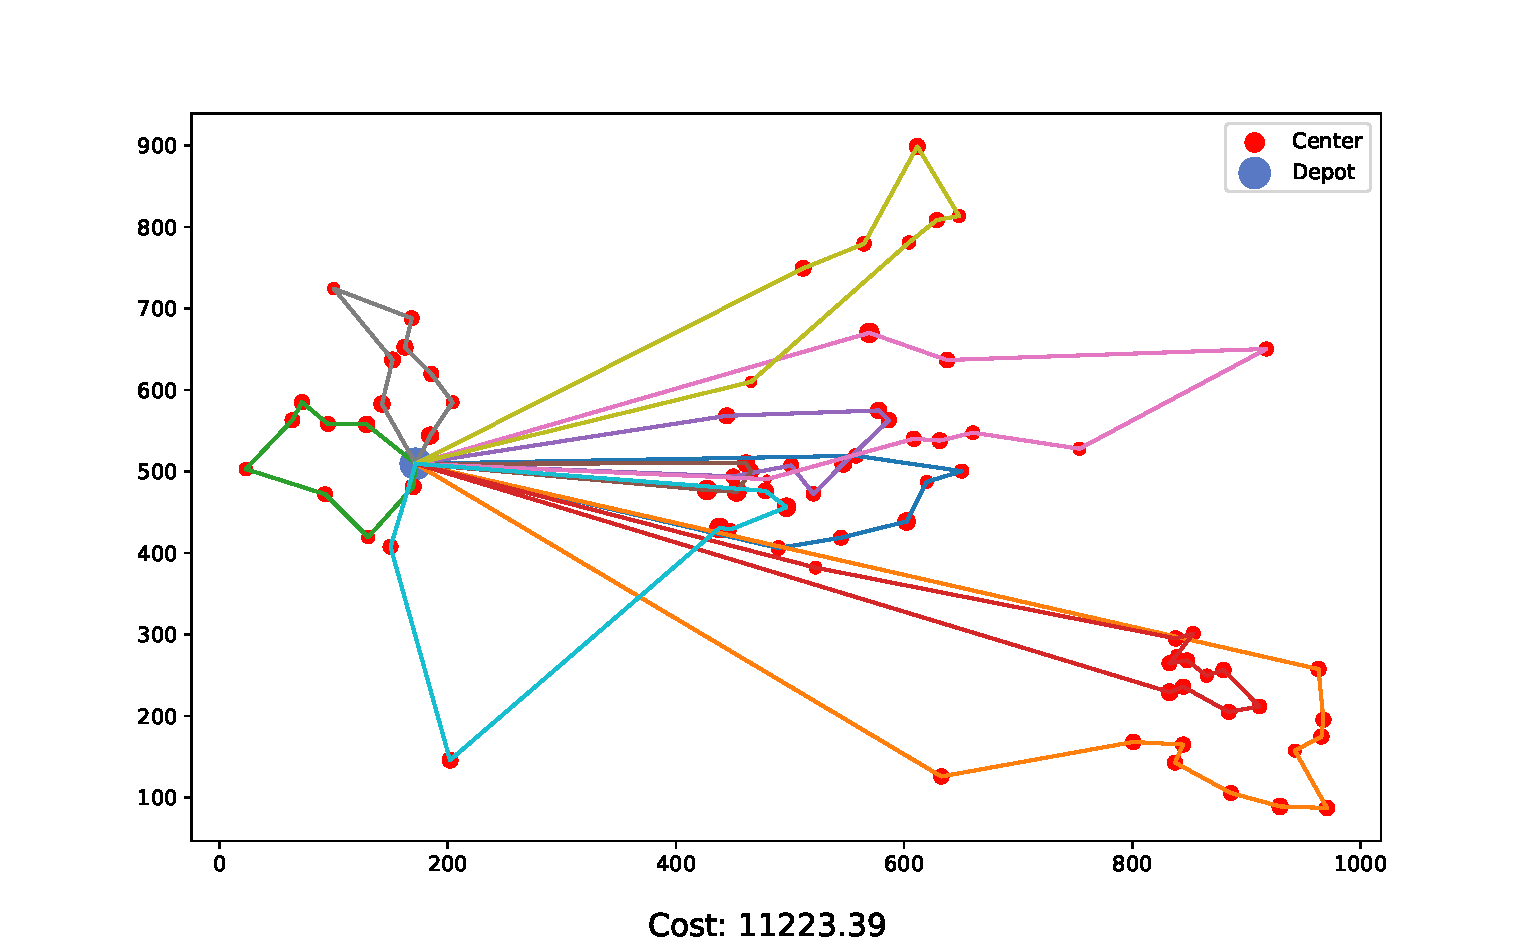
\includegraphics[width=1\columnwidth]{figures/results_poly_avg.pdf}
    \caption{method: polynomial, data: average, runtime: 7h}
  \label{fig:res-poly-avg}
\end{figure}

\begin{figure}[tb]
    \centering
    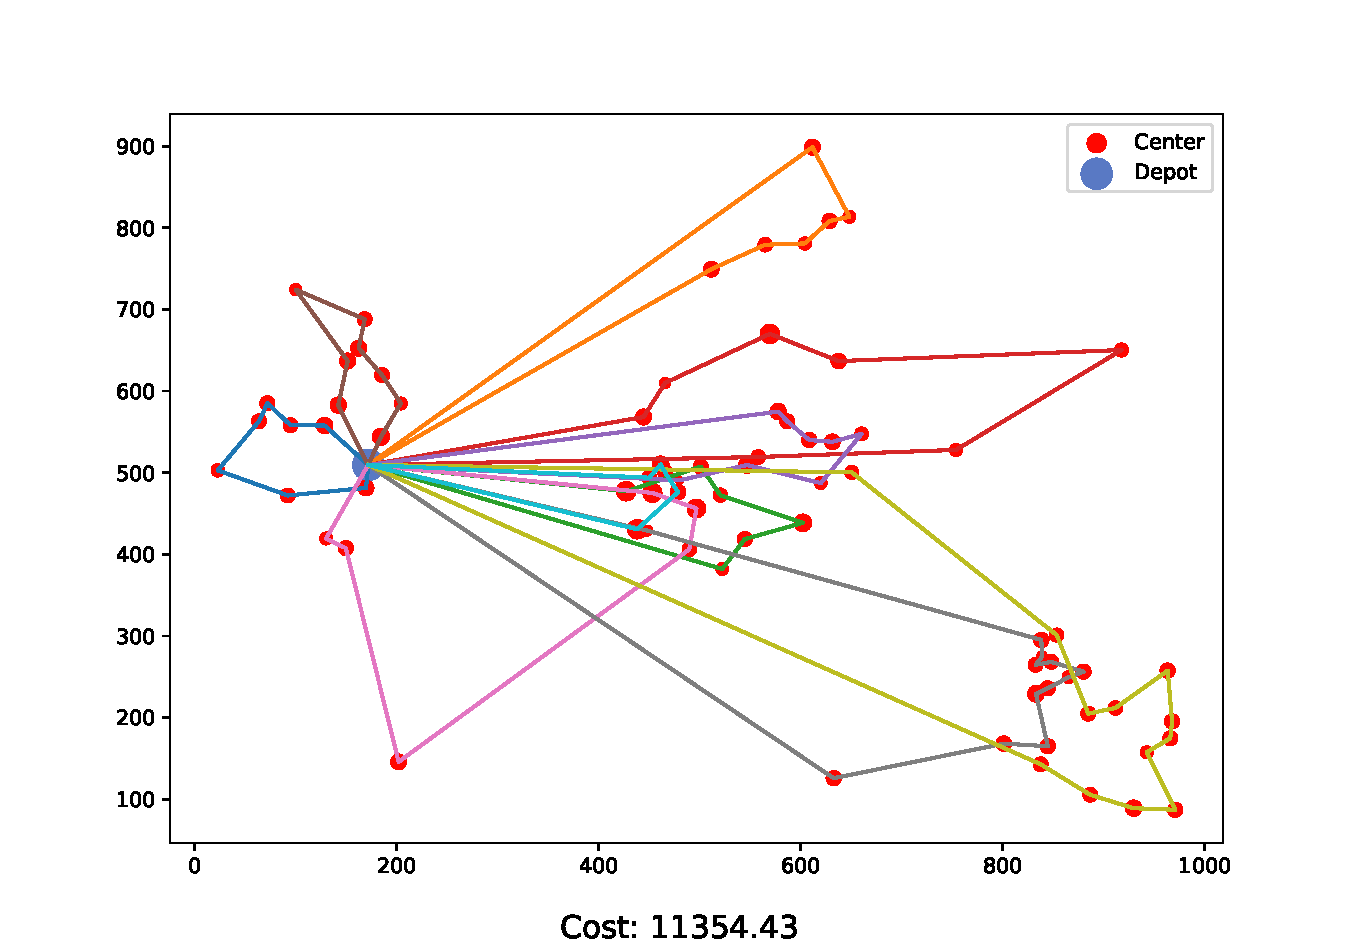
\includegraphics[width=1\columnwidth]{figures/results_poly_real.pdf}
    \caption{method: polynomial, data: real, runtime: 5h}
  \label{fig:res-poly-real}
\end{figure}
